% Supplementary material for the JFM Rapids paper "Capillary effects on the self-similar growth of immiscible Rayleigh--Taylor mixing".
% Content: derivations and simulation diagnostics from the notes ../notes/alpha_surface_tension.tex, and the mass-flux section and figure 3 moved from the paper for length.
% Figures: ../figures/fig_hinze_ratio.pdf, ../figures/fig_transition_time.pdf, ../figures/fig_alpha_transition.pdf and ../figures/fig_Rf_time.pdf from ../make_figures.ipynb; the simulation figures in ../figures/simulations/.
% Equation, section, figure and table numbers of the paper are written out (jfm.cls numbers equations by section); check them if the paper is renumbered.
% On Overleaf, add this file and its figures to the paper's project and compile it as the main document (Menu > Main document); it uses the paper's jfm.bst and jfm.bib.

\documentclass[11pt]{article}
\usepackage[a4paper, margin=25mm]{geometry}
\usepackage{amsmath}
\usepackage{graphicx}
\usepackage{newtxtext}
\usepackage{newtxmath}
\usepackage{stmaryrd}
\usepackage{natbib}
\usepackage{booktabs}
\usepackage{hyperref}
\hypersetup{
    colorlinks = true,
    urlcolor   = blue,
    citecolor  = black,
    linkcolor  = black,
}
\graphicspath{{../figures/}{../figures/simulations/}}

% numbering S1, S2, ...
\renewcommand{\thesection}{S\arabic{section}}
\renewcommand{\thefigure}{S\arabic{figure}}
\renewcommand{\thetable}{S\arabic{table}}
\renewcommand{\theequation}{S\arabic{equation}}

% notation, as in the paper
\newcommand{\avg}[1]{\langle #1\rangle}
\newcommand{\At}{\mathrm{A_t}}
\newcommand{\We}{\mathrm{We}_0}
\newcommand{\lls}{\ell_\sigma}
\newcommand{\hd}{\dot h}
\newcommand{\pd}[2]{\frac{\partial #1}{\partial #2}}

\title{Supplementary material for\\ \textit{Capillary effects on the self-similar growth of immiscible Rayleigh--Taylor mixing}}
\author{M. D. Walker and S. S. Nixon}
\date{}

\begin{document}
\maketitle

This document accompanies the paper. Sections, figures, tables and equations numbered with the prefix S belong to this document; all other references are to the paper. Sections~\ref{sec:moments} and \ref{sec:corrections} give the derivations behind \S\S\,3 and 4 of the paper, \S\,\ref{sec:hinze} the Hinze scale of the simulations, \S\,\ref{sec:terms} the terms through which surface tension can act, \S\,\ref{sec:sims} further diagnostics of the simulations, and \S\,\ref{sec:massflux} the mass-flux decomposition and the energy budget. As in the paper, RC04 and CCM04 denote \citet{Ristorcelli2004} and \citet{Cook2004}, and $h = 6 \int \bar V (1 - \bar V) \, \mathrm d z$ is the full width, with $\bar V$ the plane-averaged volume fraction of heavy fluid.

%=====================================================================
\section{Moment equations for an immiscible indicator}\label{sec:moments}

\subsection{Governing equations}\label{sec:eqs}

Following RC04, the Boussinesq form is used for the analysis; \S\,\ref{sec:massflux} treats variable density through the mass flux. With $c = +1$ in the heavy fluid and $c = -1$ in the light fluid, $\rho = \bar\rho(1 + \At c)$, and with the pressure divided by $\bar\rho$,
\begin{align}
  \pd{\mathbf u}{t} + \mathbf u \cdot \nabla \mathbf u & = -\nabla p - \At g \, c \, \mathbf e_z + \frac{\mu}{\bar\rho} \nabla^2 \mathbf u + \nabla \cdot \mathbf T^\sigma \;, \label{eq:mom} \\
  \pd{c}{t} + \mathbf u \cdot \nabla c & = 0 \, , \qquad \nabla \cdot \mathbf u = 0 \;, \label{eq:indicator}
\end{align}
where $\mathbf u = (u, v, w)$ is the velocity, $w$ its component along the upward unit vector $\mathbf e_z$ and $\mu$ the dynamic viscosity, and the capillary stress tensor is \citep{Lafaurie1994}
\begin{equation}
  \mathbf T^\sigma = \frac{\sigma}{\bar\rho} \,(\mathbf I - \hat{\mathbf n} \hat{\mathbf n}) \, \delta_s \, , \qquad \hat{\mathbf n} = \frac{\nabla c}{| \nabla c |} \;,
  \label{eq:Tsigma}
\end{equation}
with $\delta_s$ the surface delta function. Since $\nabla \cdot [(\mathbf I - \hat{\mathbf n} \hat{\mathbf n}) \, \delta_s] = \kappa \, \hat{\mathbf n} \, \delta_s$, with $\kappa = -\nabla \cdot \hat{\mathbf n}$ the curvature of the interface, the force $\mathbf f \equiv \nabla \cdot \mathbf T^\sigma = (\sigma/\bar\rho) \, \kappa \, \hat{\mathbf n} \, \delta_s$ is the continuum surface force of \citet{Brackbill1992}. Angle brackets denote averages over horizontal planes, and $c = C + c'$ with $C = \avg c$. Incompressibility and the walls give $\avg w = 0$.

\subsection{The immiscibility constraint}\label{sec:constraint}

Because $c^2 = 1$ everywhere, $\avg{c' c'} = 1 - C^2$, which is (3.1) of the paper. RC04 define the molecular mixing parameter $\theta_m = 1 - \avg{c' c'}/[(1 - C)(1 + C)]$ (their equation 4.12, in which their $c$ is the fluctuation $c'$); by (3.1) of the paper, it vanishes for immiscible fluids. Their scalar-variance equation (their equation 2.9) is then satisfied automatically, since the scalar dissipation is zero and $\avg{w c' c'} = -2 C \avg{w c'}$. The relation $\avg{c' c'}_\mathrm{o} = C_\mathrm{o}^2$ that RC04 obtain from the similarity groups (their equation 3.4) is replaced, on the mid-plane where $C = 0$, by
\begin{equation}
  \avg{c' c'}_0 = 1 \;.
  \label{eq:cc0}
\end{equation}
Here the subscript `$\mathrm{o}$' follows RC04: it marks the temporal amplitude $F_\mathrm{o}(t)$ in the self-similar form $F(z, t) = F_\mathrm{o}(t) \, f(\eta)$, which is proportional to the mid-plane value for an even profile and is set by integrals of the profile for an odd one. The amplitude $C_\mathrm{o}$ of the mean indicator is constant in the turbulent growth phase (RC04, their \S\,3) and is the growth constant in (3.6) of the paper. The subscript `$0$' on a statistic denotes its value on the mid-plane $z = 0$; on $\lambda_0$, $\tau_0$, $\We$, $\mathrm{Re}_0$ and $h_0$, it denotes initial or reference values. For a miscible flow, $\avg{c' c'}_0 = 1 - \theta_0$, with $\theta_0$ the mid-plane mixedness. This is the only place where miscibility enters the self-similar analysis.

\subsection{Mean indicator equation}\label{sec:mean}

Averaging (\ref{eq:indicator}) gives
\begin{equation}
  \pd{C}{t} + \pd{}{z} \avg{w c'} = 0
  \label{eq:mean}
\end{equation}
(RC04, their equation 2.7 without molecular diffusion). With the self-similar form $C = f_C(\eta)$, $\eta = z/h$ (RC04, their equation 3.1), integration from $-\infty$ to the mid-plane gives
\begin{equation}
  \avg{w c'}_0 = -\frac{\mathrm d}{\mathrm d t} \int_{-\infty}^0 (1 + C) \, \mathrm d z = -\frac{2}{R_f} \, \hd \, , \qquad \frac{2}{R_f} = \int_{-\infty}^0 \big(1 + f_C(\eta)\big) \, \mathrm d \eta \;.
  \label{eq:flux_mean}
\end{equation}
This corresponds to the RC04 similarity group $\avg{u_3 c}_\mathrm{o}/(\hd C_\mathrm{o})$. The integral equals $2/R_f$, with $R_f = \Delta \rho \, \hd/| \avg{\rho' w'}_0 |$ the mass-flux shape factor (\S\,\ref{sec:massflux}), because $1 + C = 2 \bar V$ and $\rho' = (\Delta \rho/2) \, c'$.

\subsection{Mid-plane groups}\label{sec:groups}

Multiplying the vertical component of (\ref{eq:mom}) by $c'$ and the indicator equation by $w$, adding and averaging gives the scalar-flux equation (3.2) of the paper (RC04, their equation 2.8; see also \citealt{Pope_book}). Let $F = -\avg{w c'}_0 = 2 \hd/R_f$ from (\ref{eq:flux_mean}). Each mid-plane term in (3.2) of the paper is normalised by $\hd^2/h$, with signs chosen so that a positive value is a sink of $F$:
\begin{equation}
  \begin{gathered}
  d_T = -\frac{h}{\hd^2} \, \pd{}{z} \avg{w w c'} \Big|_0 \, , \qquad d_N = -\frac{h}{\hd^2} \Big\langle c' \pd{p_N}{z} \Big\rangle_0 \, , \qquad d_\mu = \frac{h}{\hd^2} \, \frac{\mu}{\bar\rho} \avg{c' \nabla^2 w}_0 \;, \\
  d_\sigma = \frac{h}{\hd^2} \avg{c' (\mathcal P \mathbf f)_z}_0 \, , \qquad \hat w = \frac{\avg{w w}_0}{\hd^2} \, , \qquad f_C'(0) = h \, \pd{C}{z} \Big|_0 \;.
  \end{gathered}
  \label{eq:groups}
\end{equation}
Evaluating (3.2) of the paper on the mid-plane with these groups gives (3.5) of the paper, and its self-similar solution (3.6), with $C_\mathrm{o} = \avg{c' c'}_0 (1 - \chi_0)/\hat D$. RC04 use the half-width; for the full width, the same relation $\alpha = C_\mathrm{o}/4$ holds with $C_\mathrm{o}$ defined through $\hd^2 = \At g C_\mathrm{o} h$.

%=====================================================================
\section{Corrections to the growth equation}\label{sec:corrections}

Complete self-similarity leaves $\alpha_\infty$ independent of $\sigma$ (\S\,2 of the paper), and two further lines of analysis are possible. First, the capillary group decays but has not yet vanished; this is incomplete similarity in the sense of \citet{Barenblatt1996}, and \S\,\ref{sec:firstorder} derives the resulting correction. Second, the profile constants may be inherited from the transition. RC04 note that self-similarity holds $\avg{c' c'}_\mathrm{o}$ at its value at the start of the turbulent growth phase (their \S\,4), and the same applies to every profile constant in $C_\mathrm{o}$. During the transition, $h \sim \lambda_0$, and the capillary ratio $\lls/\lambda_0 = (2 \At \We)^{-1/2}$ is not small, so $\chi_0$ and $\hat D$ may depend on $\We$. The form of that dependence requires a closure, as RC04 state for $C_\mathrm{o}$. Within RC04, the only alternative to a capillary group that decays as $(\lls/h)^2$ is a constant one: with the capillary moment written as $\avg{c' f_z} = (\sigma/\bar\rho) \, \Gamma$ and $\Gamma_0 \propto \lls^{-2}$, it shifts $C_\mathrm{o}$ by a pure number independent of $\lambda_0$ and again gives no dependence on $\We$.

\subsection{Growth diagnostics}\label{sec:diagnostics}

Two diagnostics of $\alpha$ are in use,
\begin{equation}
  \alpha(t) \equiv \frac{\hd^2}{4 \At g h} \, , \qquad \alpha_{\rm eff}(t) \equiv \frac{\mathrm d h}{\mathrm d (\At g t^2)} = \frac{\hd}{2 \At g t} \;.
  \label{eq:alpha_defs}
\end{equation}
The first is used in the paper and in \citet{Walker2026,Walker2027_1}; the second is equation 3.8 of RC04. For immiscible fluids, the mass fraction and the volume fraction coincide pointwise in the pure phases, so the full width is the width used in \citet{Walker2026,Walker2027_1}. For the RC04 solution, written for the full width,
\begin{equation}
  h = \alpha \At g t^2 + 2 t \,(\alpha \At g h_0)^{1/2} + h_0 \;,
  \label{eq:rc_solution}
\end{equation}
$\alpha(t) = \alpha$ for all $t$, whereas $\alpha_{\rm eff} = \alpha \,[1 + (h_0/\alpha \At g t^2)^{1/2}]$ retains the virtual origin. Integrating the definition of $\alpha(t)$ gives
\begin{equation}
  \sqrt{h(t)} = \sqrt{h(0)} + \int_0^t \big(\alpha(t') \, \At g\big)^{1/2} \, \mathrm d t' \;.
  \label{eq:sqrt_h}
\end{equation}

\subsection{First-order capillary correction}\label{sec:firstorder}

By (4.1) of the paper, the capillary group is not constant but decays as a power of $h$,
\begin{equation}
  d_\sigma = \hat d_\sigma \Big(\frac{\lls}{h}\Big)^{\nu} \, , \qquad \hat d_\sigma \sim \frac{1}{2 \alpha} \, , \qquad \nu = 2 \;,
  \label{eq:dsigma_power}
\end{equation}
whereas $\avg{c' c'}_0$, $\chi_0$ and $\hat D$ take their self-similar values. For $h \gg \lls$, $d_\sigma \ll \hat D$, and the denominator of (3.6) of the paper may be expanded, $(\hat D + d_\sigma)^{-1} = \hat D^{-1} [1 - d_\sigma/\hat D + \mathcal O(d_\sigma^2)]$. This gives
\begin{equation}
  \hd^2 = \At g \, C_\mathrm{o} \, h \, \Big[1 - a_\sigma \Big(\frac{\lls}{h}\Big)^{\nu}\Big] \, , \qquad a_\sigma = \frac{\hat d_\sigma}{\hat D} > 0 \;,
  \label{eq:cap_ode}
\end{equation}
which is the modified growth equation of \S\,\ref{sec:modified} with $\nu = 2$. The sign of $a_\sigma$ follows from the restoring character of the capillary force (\S\,4 of the paper). Integrating (\ref{eq:cap_ode}) for $h \gg \lls$ (\S\,\ref{sec:integration}) gives, for the two diagnostics (\ref{eq:alpha_defs}),
\begin{align}
  \alpha(t) & = \alpha_\infty \Big[1 - a_\sigma \Big(\frac{\lls}{h}\Big)^{\nu}\Big] \;, \label{eq:alpha_t_corr} \\
  \alpha_{\rm eff}(t) & = \alpha_\infty \Big[1 - a_\sigma \, \frac{1 - \nu}{1 - 2 \nu} \Big(\frac{\lls}{h}\Big)^{\nu} - \frac{c_v}{\sqrt h} + \dots\Big] \;, \label{eq:alpha_eff_corr}
\end{align}
where $c_v$ is set by the virtual origin. In $\alpha_{\rm eff}$, the virtual-origin term decays as $h^{-1/2}$ and dominates any correction with $\nu > 1/2$; (\ref{eq:alpha_t_corr}) does not contain it. With (2.1) and (2.2) of the paper, (\ref{eq:alpha_t_corr}) reads
\begin{equation}
  \alpha(t) = \alpha_\infty \Big[1 - a_\sigma \,(2 \At \We)^{-\nu/2} \Big(\frac{\lambda_0}{h}\Big)^{\nu}\Big] = \alpha_\infty \Big[1 - a_\sigma \Big(\frac{2 \alpha}{\mathrm{We}(t)}\Big)^{\nu/2}\Big] \;,
  \label{eq:alpha_We_corr}
\end{equation}
which for $\nu = 2$ is (4.2) of the paper. For $a_\sigma > 0$, both diagnostics decrease as $\sigma$ increases.

\subsection{A modified growth equation}\label{sec:modified}

The effect of surface tension on the late-time growth can be written as a modification of the RC04 equation,
\begin{equation}
  \hd^2 = \At g C_\mathrm{o} h \Big[1 - a \Big(\frac{\lls}{h}\Big)^{\nu}\Big] \, , \qquad C_\mathrm{o} = 4 \alpha_\infty \;,
  \label{eq:mod_ode}
\end{equation}
where $a$ is a constant. Equation (\ref{eq:mod_ode}) has the form of (\ref{eq:cap_ode}) with the exponent $\nu$ left open. The Hinze-scale estimate (4.4) of the paper relates the exponent to the fractal dimension $D_s$ of the interface,
\begin{equation}
  \nu = \frac{6 q - 2}{5} = \frac{3 p - 5}{5} = \frac{7 - 3 D_s}{5} \;,
  \label{eq:mod_nu}
\end{equation}
where $q$ and $p$ are the exponents of the second-order structure function of the indicator, $\propto r^{2 q}$, and of its spectrum, $E_c(k) \propto k^{-p}$, related to $D_s$ by (6.1) of the paper. A smooth interface, $D_s = 2$, has $q = 1/2$ and $p = 2$, and gives $\nu = 1/5$. The value $(6 q - 2)/5$ follows from estimating the capillary term at the Hinze scale: substituting $\ell_H/h = K_H (\lls/h)^{6/5}$, (4.3) of the paper, into the left-hand side of (4.4) of the paper and omitting the factors of $K_H$,
\begin{equation}
  \Big(\frac{\lls}{h}\Big)^{-2/5} \Big(\frac{\lls}{h}\Big)^{6 q/5} = \Big(\frac{\lls}{h}\Big)^{(6 q - 2)/5} \;.
  \label{eq:hinze_nu}
\end{equation}
For $\nu = 1/5$, $(1 - \nu)/(1 - 2 \nu) = 4/3$, and (\ref{eq:alpha_eff_corr}) gives, with the virtual-origin term omitted,
\begin{equation}
  \alpha_{\rm eff}(h) = \frac{C_\mathrm{o}}{4} \Big[1 - \frac{4 a}{3} \Big(\frac{\lls}{h}\Big)^{1/5}\Big] \;.
  \label{eq:mod_aeff}
\end{equation}
The factor $4/3$ appears only in $\alpha_{\rm eff}$, which divides $\hd$ by the elapsed time and so retains the larger correction from earlier times; for $\alpha(t)$, the measure used in the simulations, the coefficient is $a$, as in (\ref{eq:alpha_t_corr}). In the form (\ref{eq:mod_ode}), the spectral closure (6.2) of the paper corresponds to $a < 0$ with $\nu = 3 - D_s$ or $\nu = \tfrac65 (3 - D_s)$, and the capillary-velocity form (2.3) of the paper to $\nu = 1$ and $a = -K/\alpha_\infty$.

Equation (\ref{eq:mod_ode}) offers a single description of the Weber-number dependence of $\alpha$ across all cases. Decreasing $\We$ increases $\lls \propto \sigma^{1/2}$ through (2.1) of the paper. In the simulations, this increases the growth rate and delays self-similarity, and the curves eventually converge (\S\,\ref{sec:sims}). The leading-order term of (\ref{eq:mod_ode}) is the RC04 equation and gives the standard $\alpha$. The additional term shifts $\alpha$ relative to the $\We = \infty$ case, and the shift decreases as $h$ grows, so all cases approach $\alpha_\infty$ as $h/\lls \rightarrowtriangle \infty$, consistent with complete self-similarity (\S\,2 of the paper). A shift that decreases with $h$ is what is required for the simulations at different Weber numbers to collapse onto a single curve, and, compared at equal mixing width, they do correspond to a single function of $\lls/h$ (\S\,7 of the paper).

Three points constrain the form of the correction. First, the sign: with $a > 0$, $\alpha(t)$ (\ref{eq:alpha_t_corr}) decreases as $\lls$ increases, and so does $\alpha_{\rm eff}$ (\ref{eq:alpha_eff_corr}) for $\nu < 1/2$ or $\nu > 1$, where $(1 - \nu)/(1 - 2 \nu) > 0$; the observed increase of $\alpha$ therefore requires $a < 0$. A restoring capillary force gives $a > 0$ (\S\,4 of the paper), so a negative $a$ must come from an indirect effect of surface tension on the flow structure. Second, the exponent: the fit at equal mixing width, (7.1) of the paper, has $\nu \approx 1$, whereas (\ref{eq:mod_nu}) gives $\nu \le 1/5$ for $D_s \ge 2$. Moreover, $\nu > 0$ in (\ref{eq:mod_nu}) requires $D_s < 7/3$; at $D_s = 7/3$, the term renormalises $C_\mathrm{o}$, and for the values $D_s \approx 2.6$--$2.7$ reported for scalar iso-surfaces in turbulence \citep{Sreenivasan1991}, $\nu < 0$ and the correction would grow with $h$. Third, the magnitude: with $\nu = 1$, the fit gives $\alpha - \alpha_\infty \approx 8.9 \, \lls/h$, which in the normalisation of (\ref{eq:mod_ode}) is $a \approx -8.9/\alpha_\infty \approx -250$. The correction is of order unity relative to $\alpha_\infty$ over the simulated range, and $| a |$ is much larger than unity.

\subsection{Integration of the modified growth equation}\label{sec:integration}

Let $\xi = (\lls/h)^{\nu}$. From (\ref{eq:cap_ode}), to first order in $\xi$,
\begin{equation}
  \hd = (\At g C_\mathrm{o} h)^{1/2} \Big[1 - \frac{a_\sigma}{2} \, \xi\Big] \;.
  \label{eq:int_hdot}
\end{equation}
Then $t = \int \mathrm d h/\hd$ gives, for $\nu \ne 1/2$,
\begin{equation}
  t = 2 \Big(\frac{h}{\At g C_\mathrm{o}}\Big)^{1/2} \Big[1 + \frac{a_\sigma}{2 (1 - 2 \nu)} \, \xi\Big] + t_v \;,
  \label{eq:int_t}
\end{equation}
with $t_v$ a constant of integration. Substituting (\ref{eq:int_hdot}) and (\ref{eq:int_t}) into $\alpha_{\rm eff} = \hd/(2 \At g t)$ and expanding,
\begin{equation}
  \alpha_{\rm eff} = \frac{C_\mathrm{o}}{4} \Big[1 - a_\sigma \Big(\frac12 + \frac{1}{2 (1 - 2 \nu)}\Big) \xi - \frac{c_v}{\sqrt h}\Big] = \frac{C_\mathrm{o}}{4} \Big[1 - a_\sigma \, \frac{1 - \nu}{1 - 2 \nu} \, \xi - \frac{c_v}{\sqrt h}\Big] \;,
  \label{eq:int_aeff}
\end{equation}
with $c_v = \tfrac12 t_v (\At g C_\mathrm{o})^{1/2}$, which is (\ref{eq:alpha_eff_corr}). Squaring (\ref{eq:int_hdot}) and dividing by $4 \At g h$ gives (\ref{eq:alpha_t_corr}).

%=====================================================================
\section{Hinze scale in the simulations}\label{sec:hinze}

Figure~\ref{fig:hinze} shows the Hinze scale, evaluated with the dissipation rate of the simulations \citep{Walker2027_2}, relative to the capillary length, against $h/\lls$ after the transition. For $6 \le t/\tau_0 \le 9.4$, it decreases as $h^{-0.11}$ to $h^{-0.35}$ for the three Weber numbers, around the $h^{-1/5}$ of (4.3) of the paper, and a fit with that slope gives $K_H \approx 2.3$ (\S\,4 of the paper). The dotted line marks $\ell_H = \lls$; below it, the inner cut-off of the spectral closure (\S\,6 of the paper) is $\ell_H$ rather than $\lls$. At $t = 9.4 \tau_0$, $\ell_H/\lls \approx 0.8$--$0.9$, and $\ell_H \approx 0.6$--$1.1$ times the grid spacing (\S\,\ref{sec:resolution}).

\begin{figure}[h]
  \centering
  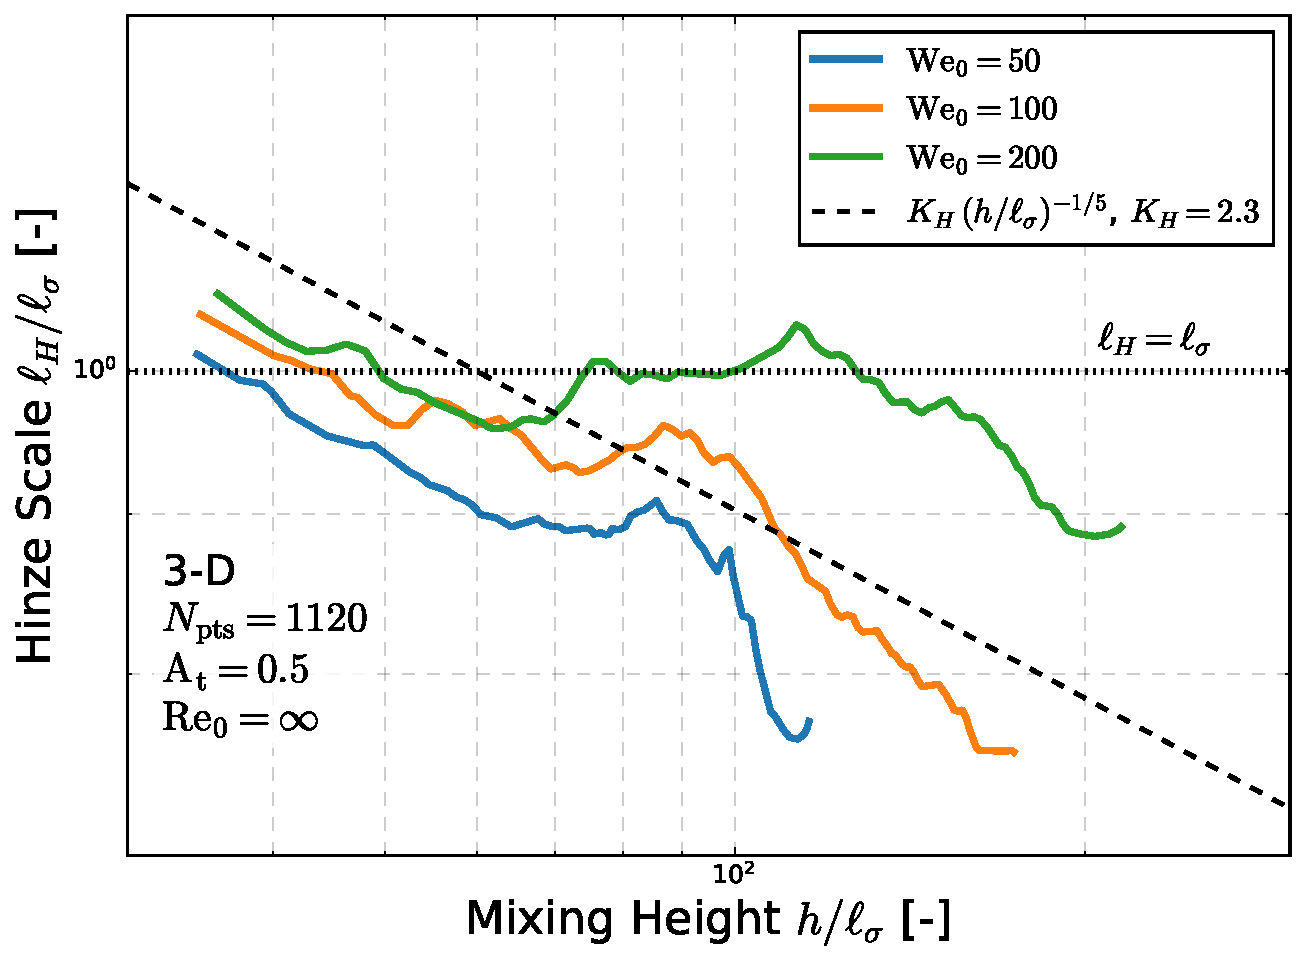
\includegraphics[width=0.6\textwidth]{fig_hinze_ratio}
  \caption{Hinze scale, evaluated with the dissipation rate of the simulations of \citet{Walker2025,Walker2026,Walker2027_1,Walker2027_2}, relative to the capillary length against $h/\lls$ after the transition, with the scaling $K_H (\lls/h)^{1/5}$ of (4.3) of the paper fitted with $K_H = 2.3$ (dashed); the dotted line marks $\ell_H = \lls$.}
  \label{fig:hinze}
\end{figure}

%=====================================================================
\section{Terms through which surface tension can act}\label{sec:terms}

By (\ref{eq:cc0}), $\avg{c' c'}_0 = 1$ for immiscible fluids, so surface tension can act on (3.6) of the paper only through the terms in table~\ref{tab:terms}. Here $D_s$ is the fractal dimension of the interface and $\ell_{\rm in}$ its inner cut-off, and the interface is assumed fractal between $\ell_H$ and $h$ when estimating the surface energy. For $2 \le D_s < 3$, the third term has the smallest exponent and is therefore the leading correction as $h/\lls \rightarrowtriangle \infty$. It is also the only one that increases $\alpha$, and it is the basis of the spectral closure of \S\,6 of the paper. In the self-similar regime, $h/\lambda_0 = \alpha_\infty (t/\tau_0)^2$, so the $\We$ exponents of (6.3) of the paper also hold at fixed $t/\tau_0$, with time factors $(t/\tau_0)^{-4/3}$ and $(t/\tau_0)^{-8/5}$ for $D_s = 7/3$ in the intermediate and asymptotic regimes.

\begin{table}[h!]
  \centering
  \begin{tabular}{lll}
    \toprule
    Term & Relative magnitude & Effect on $\alpha$ \\
    \midrule
    Capillary force in the flux budget, $d_\sigma$, (4.1) of the paper & $(\lls/h)^2$ & decrease \\
    Surface energy in the energy budget, $\Phi_\sigma$, (\ref{eq:energy}) & $(\lls/h)^{(22 - 6 D_s)/5}$ & decrease \\
    Inner cut-off of the indicator spectrum, (6.2) of the paper & $(\ell_{\rm in}/h)^{3 - D_s}$ & increase \\
    \bottomrule
  \end{tabular}
  \caption{Terms through which surface tension can modify (3.6) of the paper, with their magnitude relative to buoyancy.}
  \label{tab:terms}
\end{table}

%=====================================================================
\section{Further diagnostics of the simulations}\label{sec:sims}

Figures~\ref{fig:misc} and \ref{fig:imm} reproduce the growth parameter, mixing height and growth velocity presented in \citet{Walker2025,Walker2026}. Figure~\ref{fig:transition} and table~\ref{tab:fixed} are derived from the curves of figure~\ref{fig:imm}; the mixing height in figure~\ref{fig:imm}(\textit{b}) satisfies $h/\lambda_0 = (\hd/\sqrt{\At g \lambda_0})^2/4 \alpha$ to within about $5\,\%$.

\begin{figure}[h]
  \centering
  \begin{minipage}[t]{0.33\textwidth}\raggedright (\textit{a})\\[-2pt]
    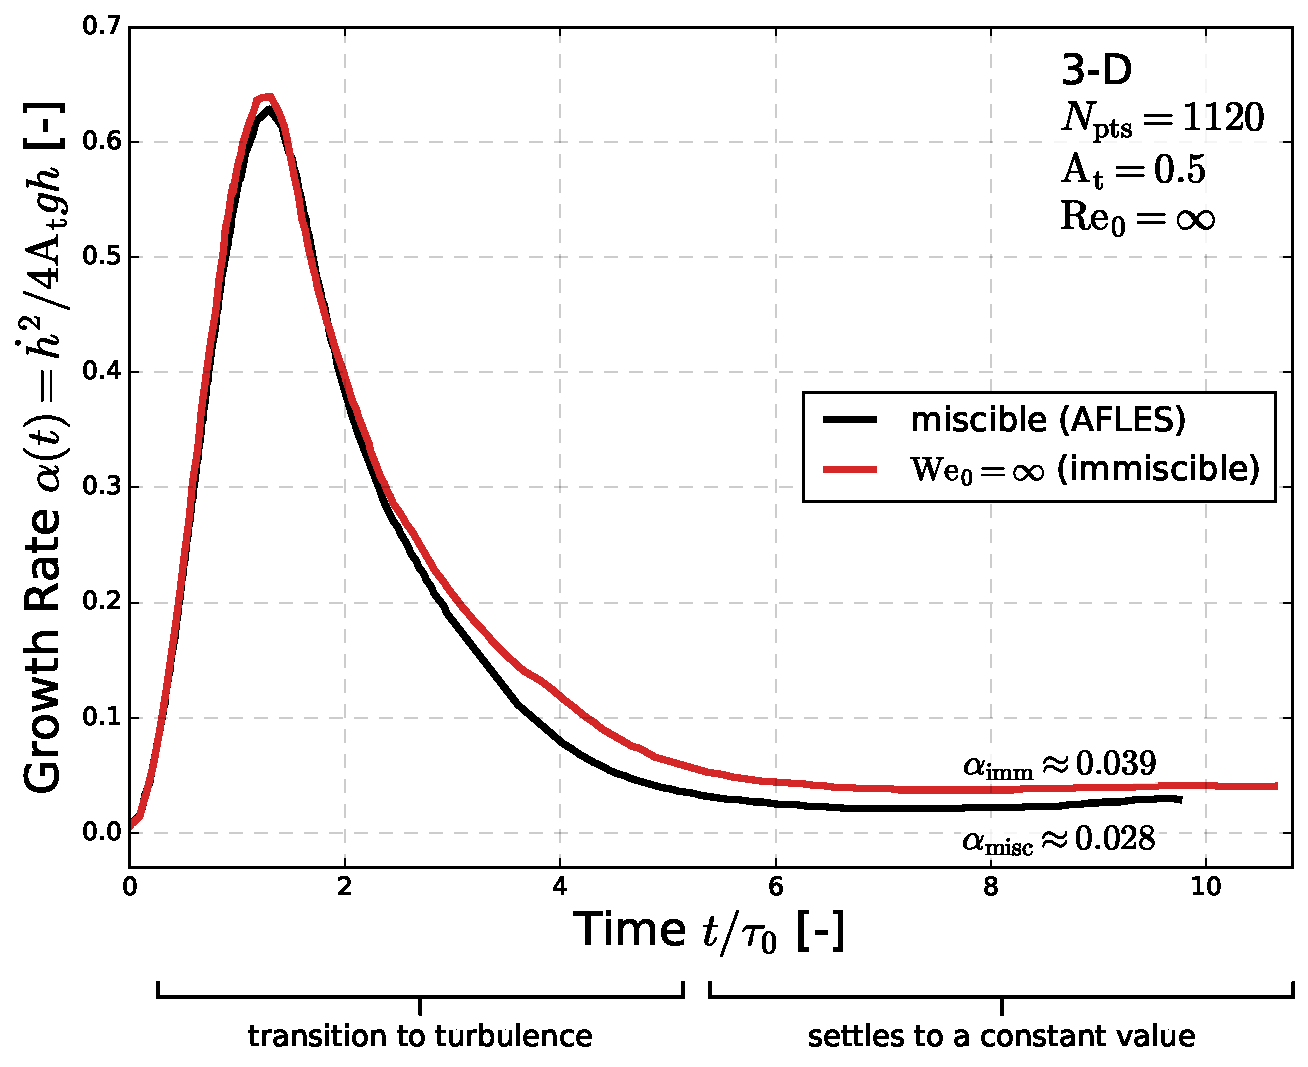
\includegraphics[width=\linewidth]{alpha_time_misc_imm}\end{minipage}\hfill
  \begin{minipage}[t]{0.333\textwidth}\raggedright (\textit{b})\\[-2pt]
    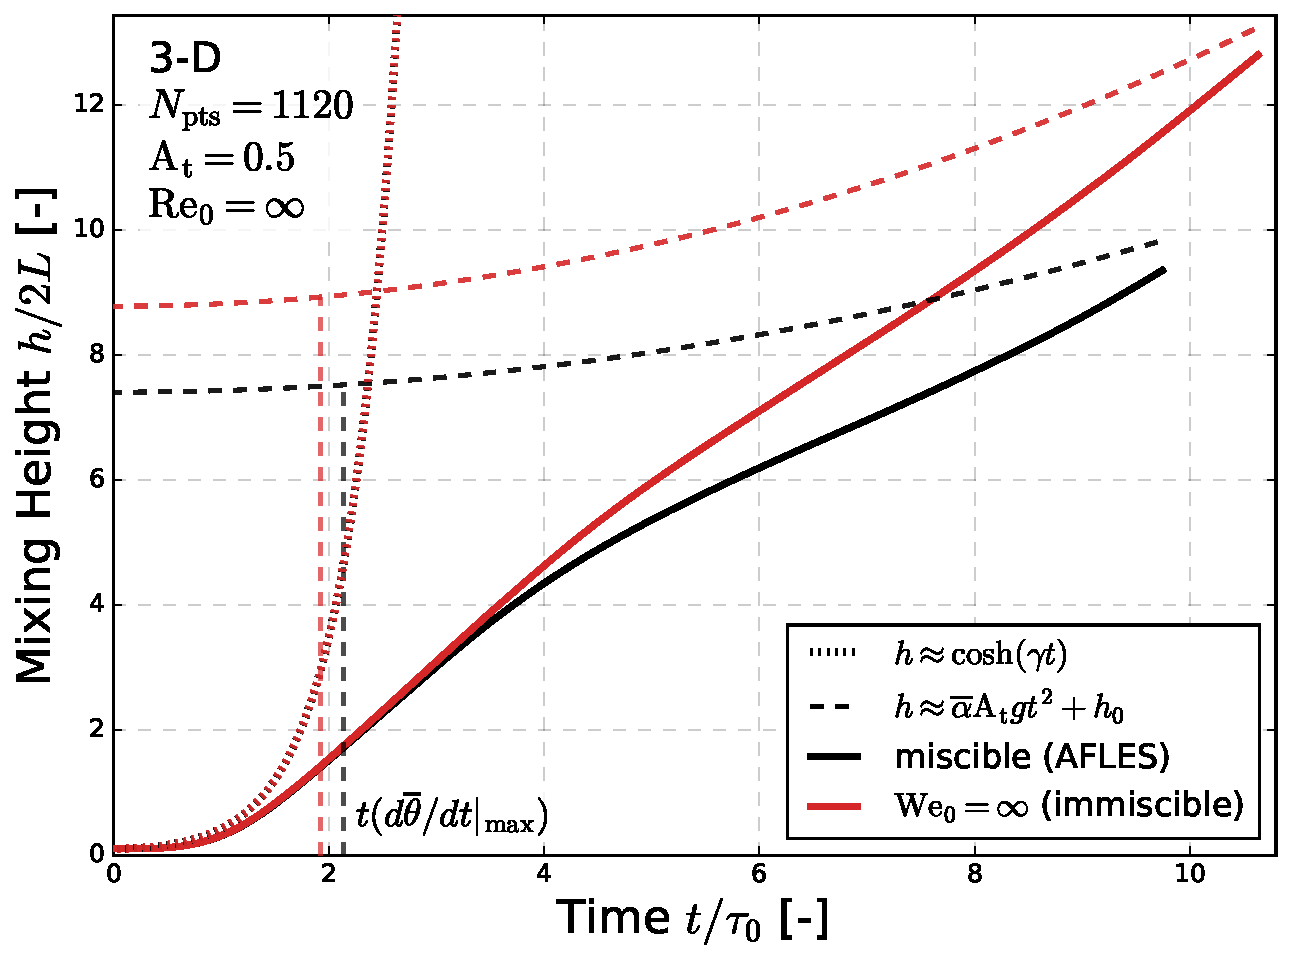
\includegraphics[width=\linewidth]{alpha_time_misc_imm_height}\end{minipage}\hfill
  \begin{minipage}[t]{0.333\textwidth}\raggedright (\textit{c})\\[-2pt]
    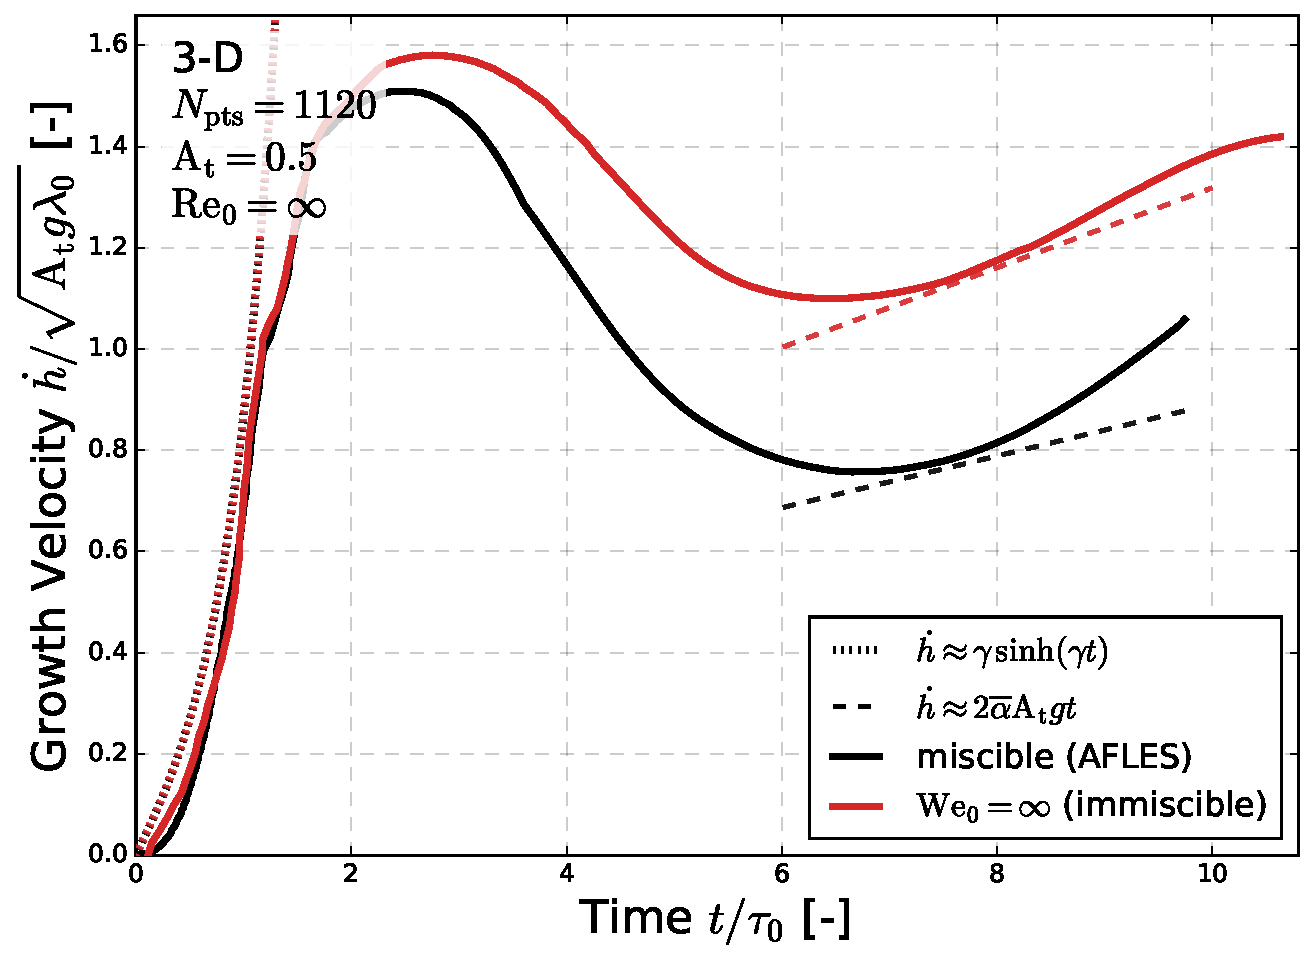
\includegraphics[width=\linewidth]{alpha_time_misc_imm_velocity}\end{minipage}
  \caption{Miscible (AFLES) and immiscible ($\We = \infty$) simulations of \citet{Walker2025,Walker2026}, with $1120^3$ points, $\At = 0.5$ and $\mathrm{Re}_0 = \infty$. (\textit{a}) Growth parameter $\alpha(t)$, (\ref{eq:alpha_defs}). (\textit{b}) Mixing height, with the linear-theory solution $h \propto \cosh(\gamma t)$ (dotted) and the fit $h \approx \bar\alpha \At g t^2 + h_0$ (dashed); vertical lines mark the time of maximum $\mathrm d \bar\theta/\mathrm d t$. (\textit{c}) Growth velocity $\hd/(\At g \lambda_0)^{1/2}$, with $\hd \propto \gamma \sinh(\gamma t)$ (dotted) and $\hd \approx 2 \bar\alpha \At g t$ (dashed).}
  \label{fig:misc}
\end{figure}

\begin{figure}[h]
  \centering
  \begin{minipage}[t]{0.33\textwidth}\raggedright (\textit{a})\\[-2pt]
    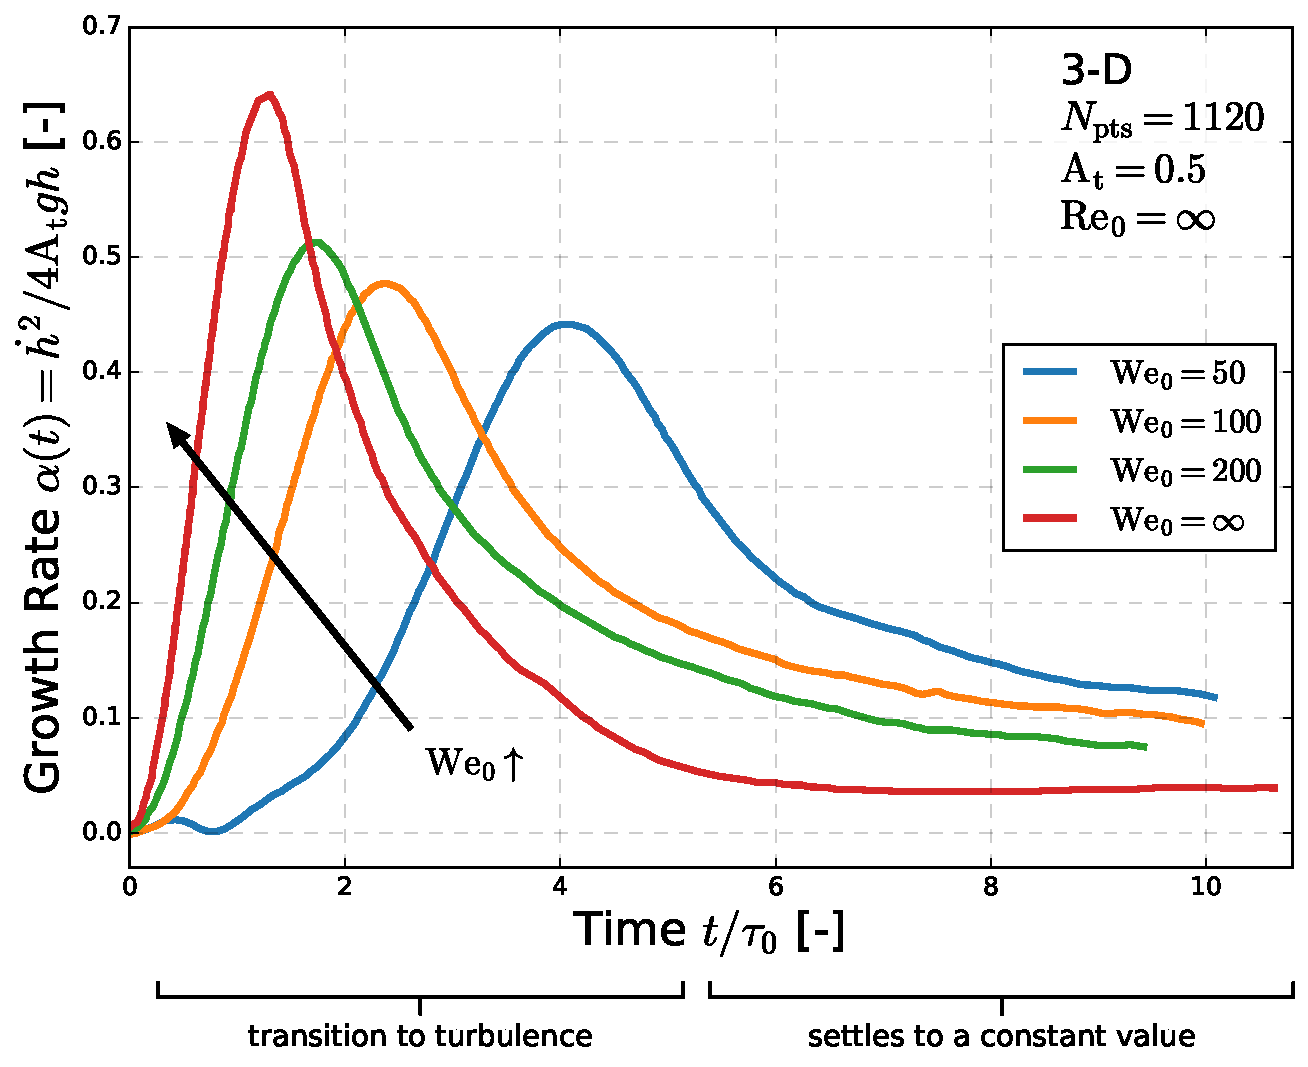
\includegraphics[width=\linewidth]{immiscible_alpha_time}\end{minipage}\hfill
  \begin{minipage}[t]{0.333\textwidth}\raggedright (\textit{b})\\[-2pt]
    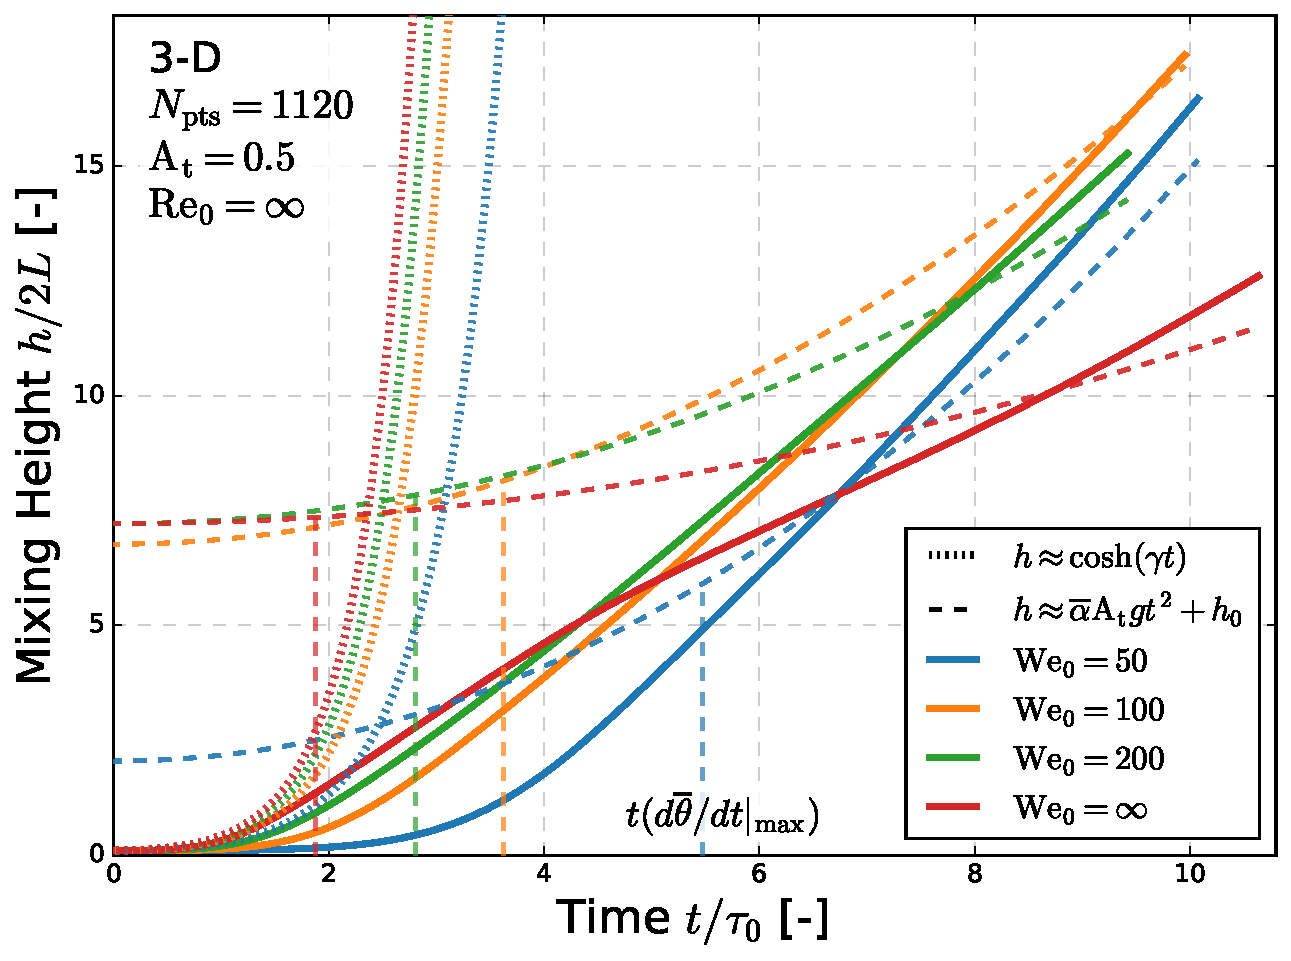
\includegraphics[width=\linewidth]{immiscible_alpha_time_height}\end{minipage}\hfill
  \begin{minipage}[t]{0.333\textwidth}\raggedright (\textit{c})\\[-2pt]
    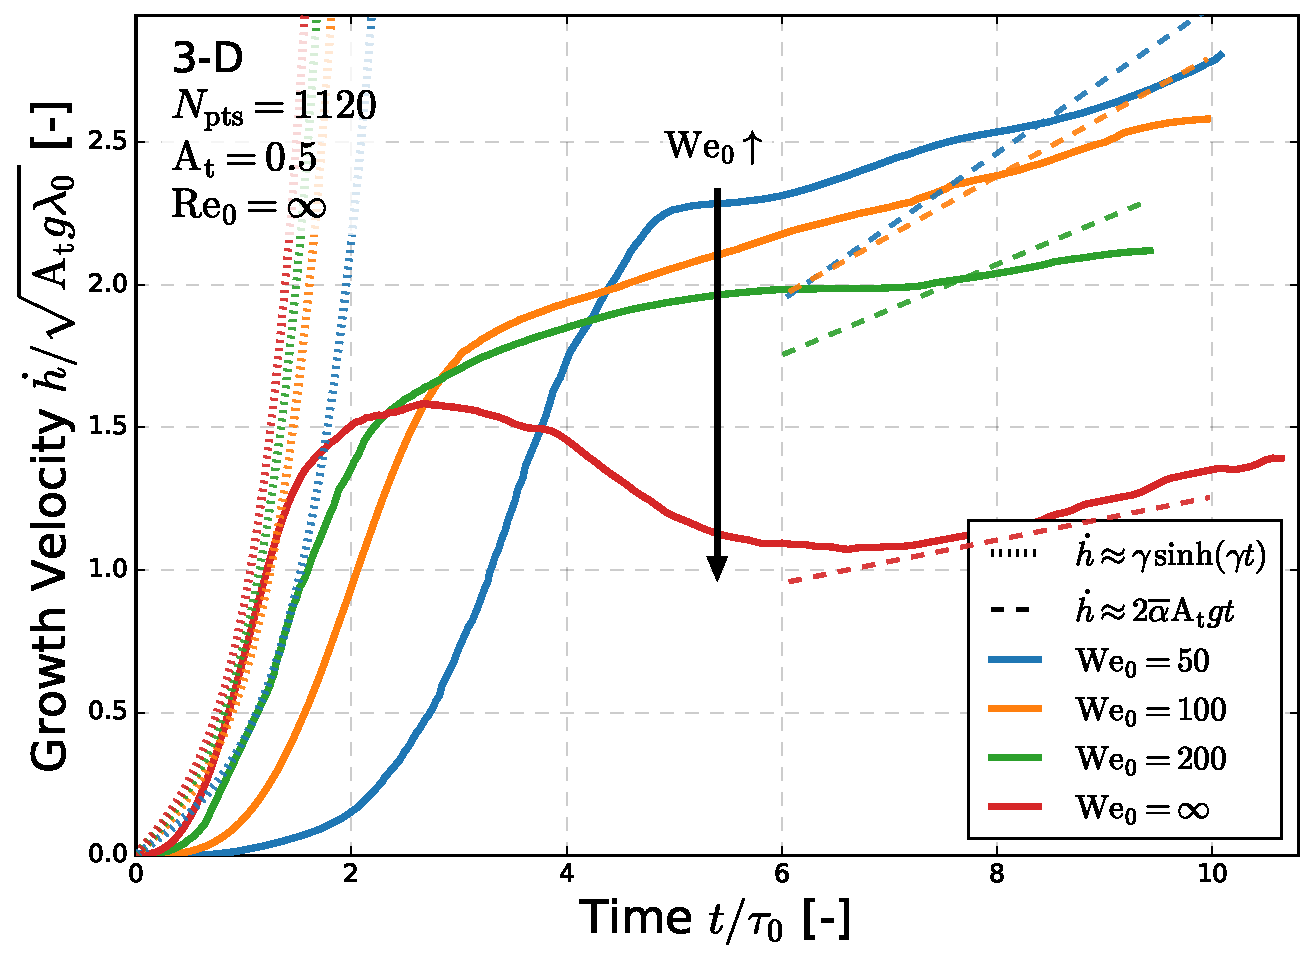
\includegraphics[width=\linewidth]{immiscible_alpha_time_velocity}\end{minipage}
  \caption{Immiscible simulations of \citet{Walker2025,Walker2026} at $\We = 50$, $100$, $200$ and $\infty$, with $1120^3$ points, $\At = 0.5$ and $\mathrm{Re}_0 = \infty$; panels and line styles as in figure~\ref{fig:misc}.}
  \label{fig:imm}
\end{figure}

\subsection{Miscible and immiscible cases}\label{sec:misc}

Figure~\ref{fig:misc} compares the miscible and immiscible cases without surface tension. The two follow the same linear and early nonlinear growth (figure~\ref{fig:misc}\textit{b,c}) and the same peak in $\alpha(t)$ near $t \approx 1.3 \tau_0$ (figure~\ref{fig:misc}\textit{a}). After the transition, the immiscible layer grows faster, and $\alpha(t)$ settles at $\alpha \approx 0.039$, compared with $\alpha \approx 0.028$ in the miscible case. In both cases, the late-time growth velocity increases approximately linearly in time (figure~\ref{fig:misc}\textit{c}), as expected for quadratic growth.

\subsection{Transition}\label{sec:transition}

Decreasing $\We$ delays the transition and lowers the peak of $\alpha(t)$ (figure~\ref{fig:imm}\textit{a}). The time $t_\theta$ of maximum $\mathrm d \bar\theta/\mathrm d t$, marked in figure~\ref{fig:imm}(\textit{b}), and the time $t_{\rm peak}$ of peak $\alpha$ both increase linearly with $\We^{-1}$, that is, linearly with $\sigma$ (figure~\ref{fig:transition}\textit{a}):
\begin{equation}
  \frac{t_\theta}{\tau_0} \approx 1.88 + \frac{179}{\We} \, , \qquad \frac{t_{\rm peak}}{\tau_0} \approx 1.15 + \frac{139}{\We} \;,
  \label{eq:t_transition}
\end{equation}
with root-mean-square deviations of $0.03$ and $0.13$ over the four cases, including $\We = \infty$. A delay linear in $\sigma$ is the form expected from the first-order capillary correction to the linear growth rate, $\gamma^2 = \At g k \,(1 - k^2 \lls^2)$. Aligned at $t_\theta$ (figure~\ref{fig:transition}\textit{b}), the finite-$\We$ curves nearly coincide for $(t - t_\theta)/\tau_0 \lesssim 3$; the ratio of the largest to the smallest $\alpha$ among $\We = 50$--$200$ rises from $1.04$ at $(t - t_\theta)/\tau_0 = 2$ to $1.32$ at $4.5$, and the ratio to $\We = \infty$ from $1.3$ to $2.8$. \citet{Cook2001} found that a progress variable brings cases with different initial conditions into closer agreement than time does, and RC04 attribute this to the virtual origin.

\begin{figure}[h]
  \centering
  \begin{minipage}[t]{0.478\textwidth}\raggedright (\textit{a})\\[-2pt]
    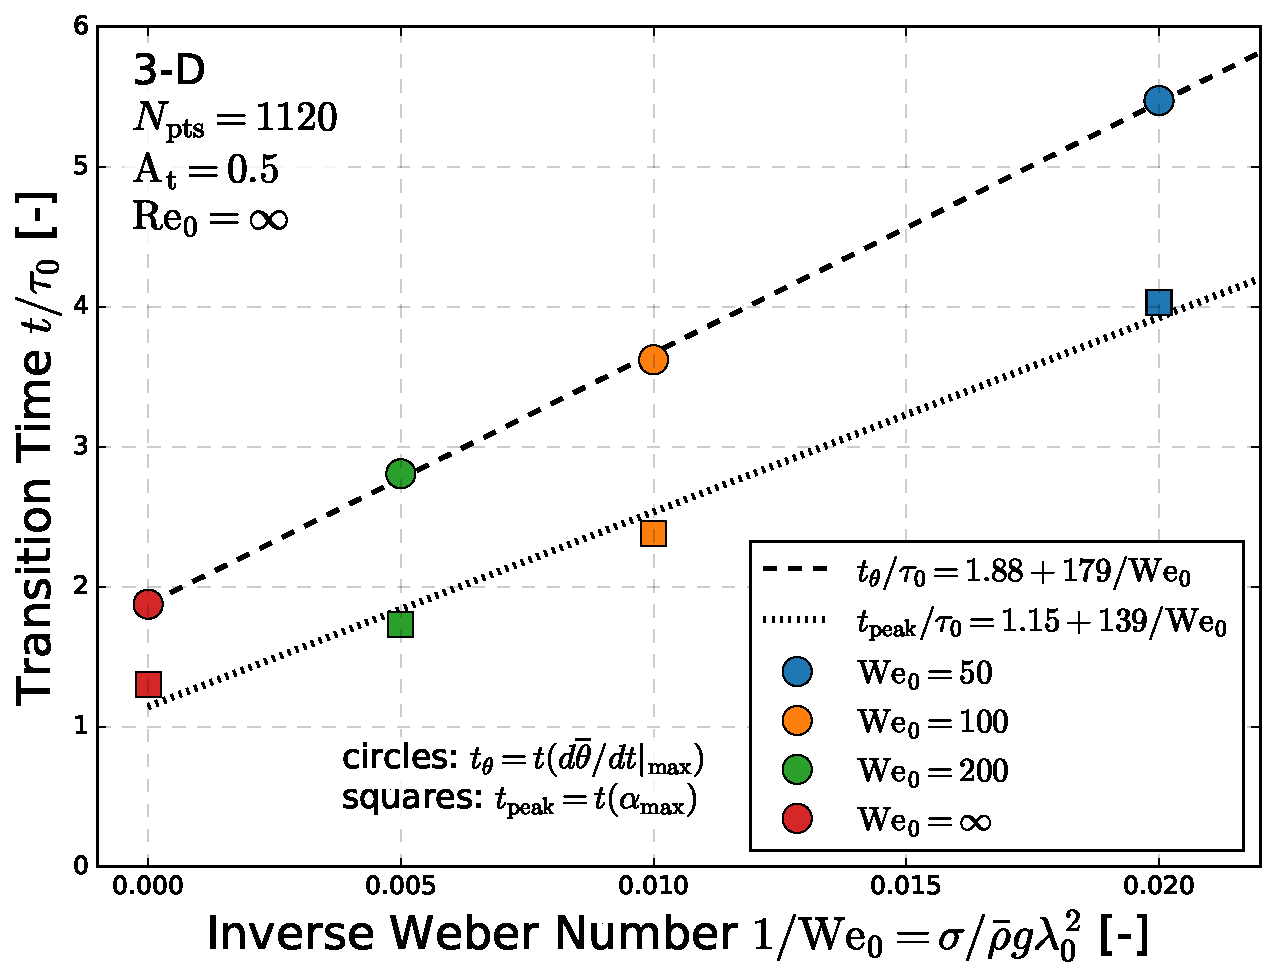
\includegraphics[width=\linewidth]{fig_transition_time}\end{minipage}\hfill
  \begin{minipage}[t]{0.49\textwidth}\raggedright (\textit{b})\\[-2pt]
    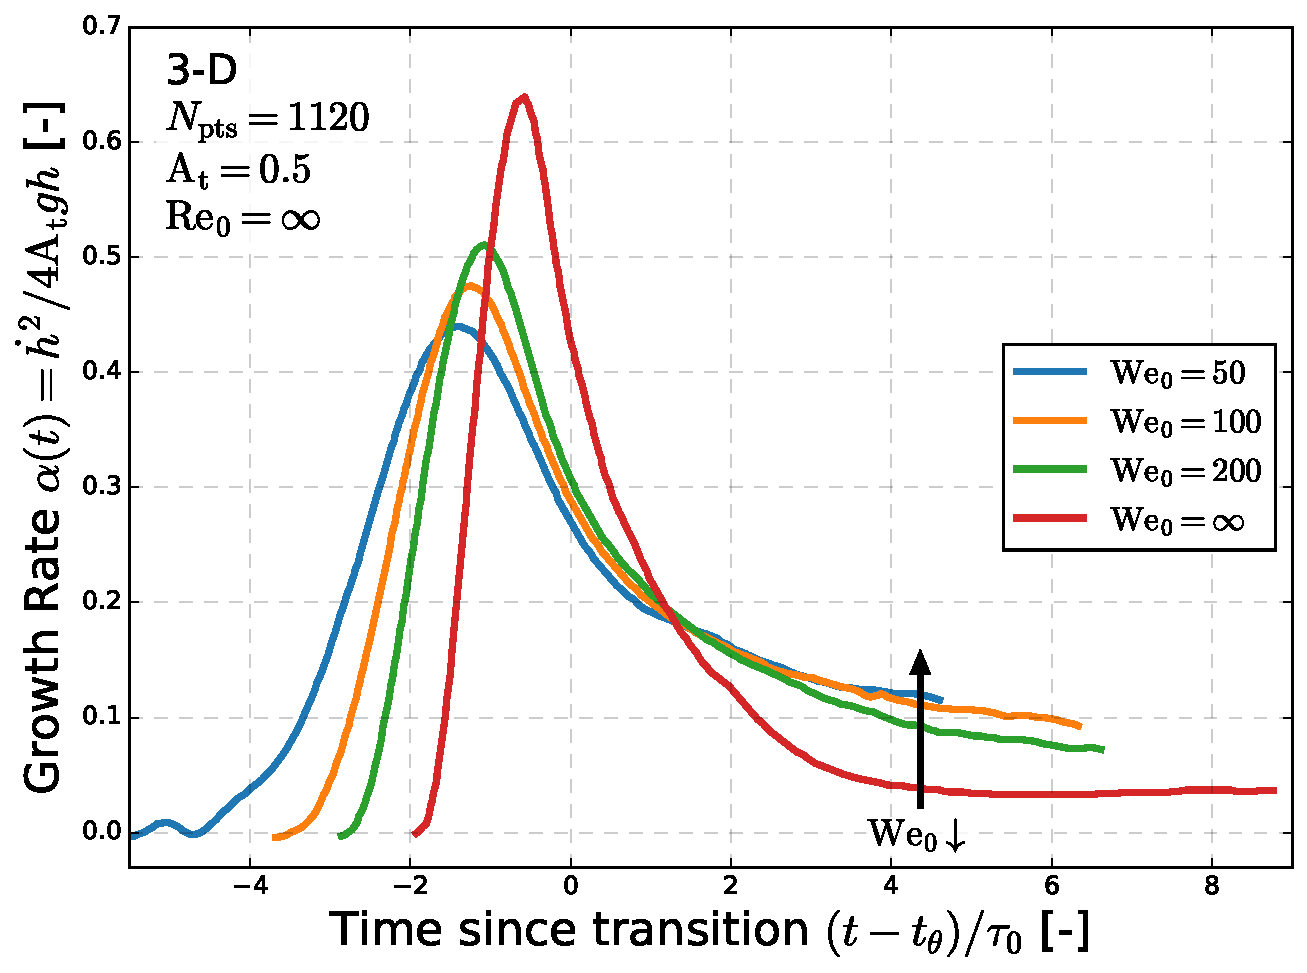
\includegraphics[width=\linewidth]{fig_alpha_transition}\end{minipage}
  \caption{(\textit{a}) Transition time against $1/\We$: time of maximum $\mathrm d \bar\theta/\mathrm d t$ (circles) and of peak $\alpha$ (squares), with the fits (\ref{eq:t_transition}). (\textit{b}) Growth parameter against time since $t_\theta$.}
  \label{fig:transition}
\end{figure}

\subsection{Comparison at fixed time}\label{sec:fixed}

Table~\ref{tab:fixed} lists the ratio $\alpha(\We = 50)/\alpha(\We = 200)$ at fixed $t/\tau_0$ and the corresponding effective power law. At $t \approx 10 \tau_0$, this is close to the fit $\alpha \approx 0.49 \, \We^{-0.35}$ of \citet{Walker2026}. The form $\alpha \approx \alpha_\infty + K \We^{-1/2}$ also fits at any single time, with $\alpha_\infty \approx 0.030$--$0.035$, but $K$ drops from $1.2$ at $6 \tau_0$ to $0.62$ at $9.4 \tau_0$. The exponent obtained at fixed time is therefore not a property of the flow; it depends on when the simulations are compared (figure~3\textit{b} of the paper).

\begin{table}[h!]
  \centering
  \begin{tabular}{ccc}
    \toprule
    $t/\tau_0$ & $\alpha(\We = 50)/\alpha(\We = 200)$ & Effective scaling \\
    \midrule
    6.0 & 1.89 & $\We^{-0.46}$ \\
    6.5 & 1.80 & $\We^{-0.43}$ \\
    7.5 & 1.84 & $\We^{-0.44}$ \\
    8.5 & 1.66 & $\We^{-0.37}$ \\
    9.4 & 1.68 & $\We^{-0.38}$ \\
    \bottomrule
  \end{tabular}
  \caption{Growth parameter compared at fixed time, from the curves of figure~\ref{fig:imm}(\textit{a}).}
  \label{tab:fixed}
\end{table}

\subsection{Resolution of the capillary scale}\label{sec:resolution}

The capillary length is close to the grid spacing in these simulations. With $\lambda_0 = L/k_{\max} \approx 1.02$\,cm and $\Delta x = L/N_\mathrm{pts} \approx 0.114$\,cm, where $L$ is the domain width, $k_{\max}$ the largest initial mode number and $N_\mathrm{pts} = 1120$, $\lls/\Delta x = 1.26$, $0.89$ and $0.63$ for $\We = 50$, $100$ and $200$, and the linear cut-off wavelength $\lls$ spans $4$--$8 \, [\Delta x]$. That the excess is a single function of $\lls/h$, (7.1) of the paper, indicates that, over the simulated range, the late-time effect of surface tension is organised by $\lls$ even though $\lls$ is comparable to the grid spacing. The Hinze scale is of the same size (\S\,\ref{sec:hinze}). The limit of drop breakup at the grid scale in these simulations is analysed with a geometric model by \citet{Walker2027_2}.

%=====================================================================
\section{Mass flux and energy budget}\label{sec:massflux}

The mass-flux relation of CCM04 indicates where the indirect effect resides. For incompressible phases, $\avg \rho = \rho_\ell + \Delta \rho \, \bar V$, and mean continuity gives
\begin{equation}
  \Delta \rho \, \pd{\bar V}{t} = -\pd{}{z} \avg{\rho w} \;.
  \label{eq:continuity}
\end{equation}
Differentiating the definition of $h$ and integrating by parts, with $\avg{\rho w} \rightarrowtriangle 0$ as $| z | \rightarrowtriangle \infty$, and with $\avg w = 0$, so that $\avg{\rho w} = \avg{\rho' w'}$,
\begin{equation}
  \hd = -\frac{12}{\Delta \rho} \int_{-\infty}^{\infty} \avg{\rho' w'} \, \pd{\bar V}{z} \, \mathrm d z \;.
  \label{eq:hdot_flux}
\end{equation}
This is the full-width counterpart of the CCM04 relation for their entrainment length $h_C = 4 \int_{-\infty}^0 \bar V \, \mathrm d z$ (their equations 3.5 and 7.3), which they approximate as $\hd_C \approx -4 \avg{\rho w}_0/\Delta \rho$ (their equation 7.4). For a self-similar profile, $\avg{\rho w}_0 = -\Delta \rho \,(\mathrm d/\mathrm d t) \int_{-\infty}^0 \bar V \, \mathrm d z$, so the shape factor $R_f = \Delta \rho \, \hd/| \avg{\rho' w'}_0 |$ depends only on the shape of $\bar V$:
\begin{equation}
  R_f = \frac{h}{\int_{-\infty}^0 \bar V \, \mathrm d z} = \frac{4 h}{h_C} =
  \begin{cases}
  8 & \text{linear profile} \;, \\
  6 \sqrt 2 \approx 8.49 & \text{error-function profile} \;, \\
  6/\ln 2 \approx 8.66 & \text{hyperbolic-tangent profile} \;.
  \end{cases}
  \label{eq:Rf_values}
\end{equation}
The value $R_f = 4$ corresponds to the entrainment length of CCM04. The scaling ratio of \citet{Walker2026,Walker2027_1} uses the half-width $h/2$ and equals $R_f/2$. Without surface tension, $R_f$ rises into the self-similar range at late times, with a mean of $8.0$ over $8 \le t/\tau_0 \le 9.4$, the value for a linear profile; with surface tension it settles at $9.7$--$10.7$, above that range, and in the miscible case it is still increasing (figure~\ref{fig:Rf} and table~\ref{tab:decomp}).

\begin{figure}[h]
  \centering
  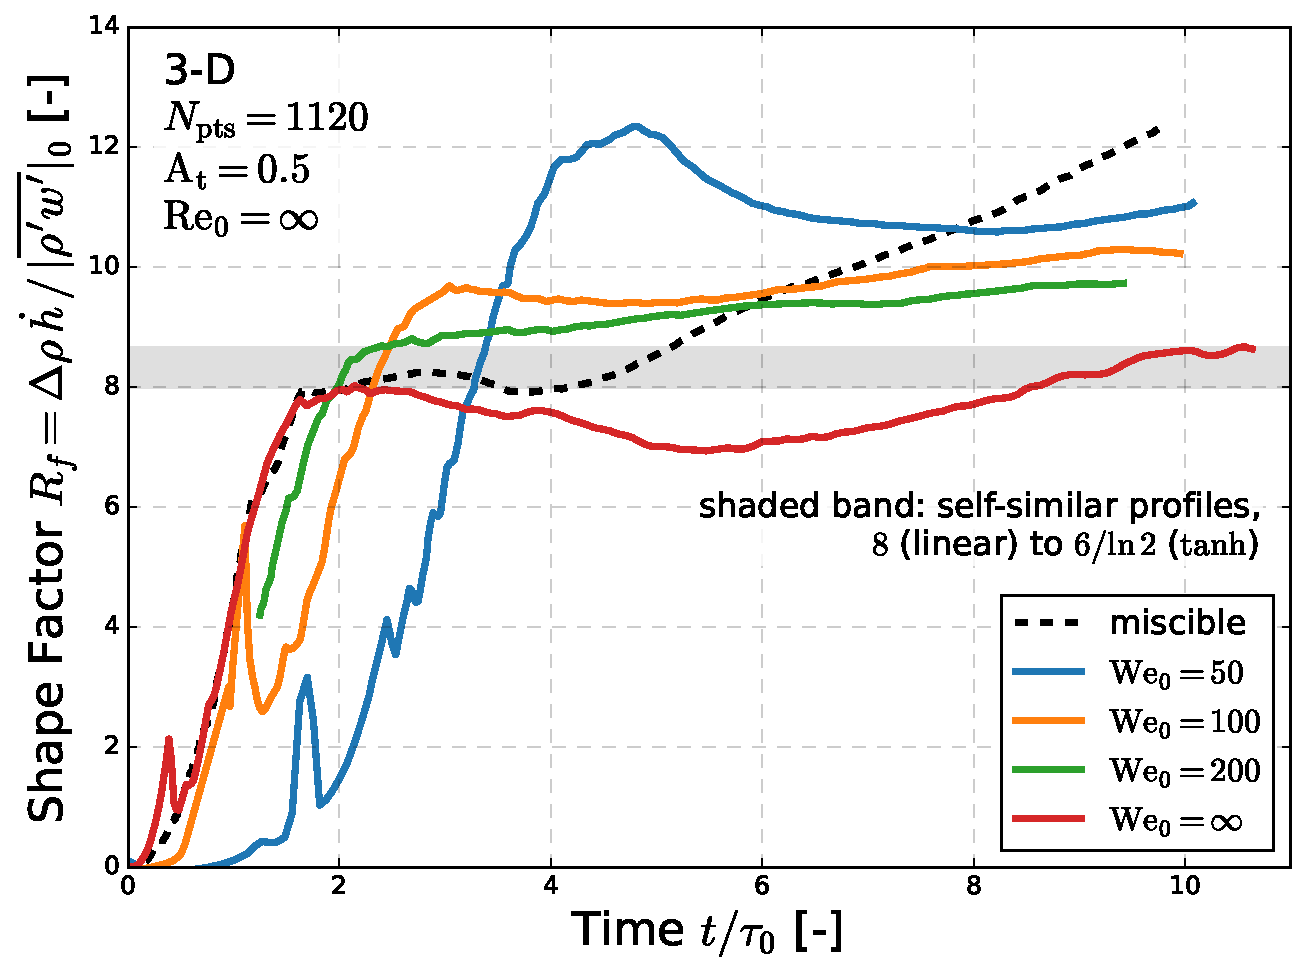
\includegraphics[width=0.6\textwidth]{fig_Rf_time}
  \caption{Mass-flux shape factor $R_f = \Delta \rho \, \hd/| \avg{\rho' w'}_0 |$ for the full width in the simulations of \citet{Walker2025,Walker2026,Walker2027_1}, twice the scaling ratio of \citet{Walker2026,Walker2027_1}; the grey band marks the self-similar values (\ref{eq:Rf_values}), from $8$ for a linear profile to $6/\ln 2$ for a hyperbolic-tangent profile.}
  \label{fig:Rf}
\end{figure}

Following CCM04 (their equation 7.5), write $\avg{\rho' w'}_0 = -C_r \rho_{\rm rms} w_{\rm rms}$, with $\rho_{\rm rms} = \Delta \rho \,[\bar V_0 (1 - \bar V_0)(1 - \theta_0)]^{1/2}$, where $\theta_0$ is the mid-plane mixedness, and define $\mathrm{Fr}_0^2 = w_{\rm rms}^2/\At g h$. With $\bar V_0 = 1/2$, the definitions of $\alpha(t)$ and $R_f$ give
\begin{equation}
  \alpha = \frac{R_f^2}{16} \, C_r^2 \,(1 - \theta_0) \, \mathrm{Fr}_0^2 \;.
  \label{eq:decomp}
\end{equation}
The effective Atwood number of CCM04 (their equation 3.14) is $\mathrm{A}_\mathrm{eff} = \At (1 - \theta_0)^{1/2}$ in this notation. Their closure $w_{\rm rms} = C_w (\mathrm{A}_\mathrm{eff} g h)^{1/2}$ (their equation 7.8) gives $\mathrm{Fr}_0^2 = C_w^2 (1 - \theta_0)^{1/2}$ and hence
\begin{equation}
  \alpha = \frac{R_f^2}{16} \, C_r^2 C_w^2 \,(1 - \theta_0)^{3/2} = \frac{R_f^2}{16} \, C_r^2 C_w^2 \Big(\frac{\mathrm{A}_\mathrm{eff}}{\At}\Big)^3 \;,
  \label{eq:cook_closure}
\end{equation}
which reduces to equation 7.12 of CCM04 for $R_f = 4$.

Table~\ref{tab:decomp} applies (\ref{eq:decomp}) to the simulations of \citet{Walker2027_1,Walker2027_2}, averaged over $8 \le t/\tau_0 \le 9.4$, with $\theta_0$ obtained from the mid-plane density fluctuation, $1 - \theta_0 = (2 \rho_{\rm rms}/\Delta \rho)^2$. Between $\We = 50$ and $\We = \infty$, the factor $3.84$ in $\alpha$ splits as $1.76$ from $R_f^2$, $1.49$ from the purity $1 - \theta_0$ and $1.46$ from $C_r^2 \mathrm{Fr}_0^2$; the three factors are comparable at every $\We$, and $R_f^2$ is the largest. Between $\We = \infty$ and the miscible case, the factor $1.51$ splits as $0.50 \times 4.25 \times 0.71$. The closure (\ref{eq:cook_closure}) would predict $4.25^{3/2} \approx 8.8$ for the latter factor, and a closure linear in $1 - \theta_0$ with the other constants fixed would predict $4.3$; the purity alone overpredicts the difference between miscible and immiscible growth. The same closure underpredicts the increase with surface tension, $1.82$ against $3.84$ at $\We = 50$. The immiscible case without surface tension has a higher purity than the miscible case but the lowest $R_f$ and $C_r \mathrm{Fr}_0$ of all five cases. Surface tension therefore raises $\alpha$ through all three factors: the shape factor of the mid-plane flux, the purity, and $C_r \mathrm{Fr}_0$, the correlation and vertical velocity of the mid-plane flux. Together they are the indirect effect required in \S\,5 of the paper.

\begin{table}[h!]
  \centering
  \def~{\hphantom{0}}
  \small
  \setlength{\tabcolsep}{3pt}
  \begin{tabular}{lccccccccccc}
    \toprule
     & \multicolumn{5}{c}{Late-time values} & & \multicolumn{5}{c}{Ratio to $\We = \infty$} \\
    \cmidrule(lr){2-6} \cmidrule(lr){8-12}
    Case & $\alpha$ & $R_f$ & $\theta_0$ & $C_r^2 \mathrm{Fr}_0^2$ & $C_r \mathrm{Fr}_0$ & & $\alpha$ & $R_f^2$ & $1 - \theta_0$ & $C_r^2 \mathrm{Fr}_0^2$ & $(1 - \theta_0)^{3/2}$ \\
    \midrule
    $\We = 50$ & 0.132 & 10.7 & 0.10 & 0.0206 & 0.144 & & 3.84 & 1.76 & 1.49 & 1.46 & 1.82 \\
    $\We = 100$ & 0.105 & 10.2 & 0.13 & 0.0189 & 0.138 & & 3.07 & 1.60 & 1.43 & 1.34 & 1.72 \\
    $\We = 200$ & 0.078 & ~9.7 & 0.19 & 0.0166 & 0.129 & & 2.27 & 1.45 & 1.34 & 1.17 & 1.54 \\
    $\We = \infty$ & 0.034 & ~8.0 & 0.40 & 0.0141 & 0.119 & & 1 & 1 & 1 & 1 & 1 \\
    Miscible & 0.023 & 11.4 & 0.86 & 0.0198 & 0.141 & & 0.66 & 2.00 & 0.24 & 1.40 & 0.11 \\
    \bottomrule
  \end{tabular}
  \caption{Decomposition (\ref{eq:decomp}) of the growth parameter, averaged over $8 \le t/\tau_0 \le 9.4$, with $R_f$ for the full width, $\theta_0$ from the mid-plane density fluctuation and $C_r^2 \mathrm{Fr}_0^2 = 16 \alpha/[R_f^2(1 - \theta_0)]$. The last column is the ratio predicted by the CCM04 closure, $\alpha \propto (1 - \theta_0)^{3/2}$.}
  \label{tab:decomp}
\end{table}

The energy budget constrains the sign in the same way. Let $P_{\rm rel} = c_P \, \Delta \rho \, g h^2$ be the released potential energy per unit horizontal area, with $c_P = 1/24$ for a linear profile, $K_E = c_K \bar\rho \, \hd^2 h$ the kinetic energy per unit area, $E_\varepsilon$ the dissipated energy and $S(t)$ the interface area per unit horizontal area. Conservation of energy, $P_{\rm rel} = K_E + E_\varepsilon + \sigma (S - 1)$, together with $\hd^2 = 4 \alpha \At g h$, gives
\begin{equation}
  \alpha = \frac{c_P}{2 c_K} \, \frac{K_E}{P_{\rm rel}} = \frac{c_P}{2 c_K} \,(1 - \Phi_\varepsilon - \Phi_\sigma) \, , \qquad \Phi_\varepsilon = \frac{E_\varepsilon}{P_{\rm rel}} \, , \quad \Phi_\sigma = \frac{\sigma (S - 1)}{P_{\rm rel}} \ge 0 \;.
  \label{eq:energy}
\end{equation}
The surface energy lowers $\alpha$, so an increase of $\alpha$ with $\sigma$ must come from a smaller dissipated fraction $\Phi_\varepsilon$ or from a change in the profile ratio $c_P/c_K$. At $\mathrm{Re}_0 = \infty$, $\Phi_\varepsilon$ is the numerical dissipation of the scheme \citep{Cook2007,Brill2025}. With the interface fractal between $\ell_H$ and $h$, $\Phi_\sigma \propto (\lls/h)^{(22 - 6 D_s)/5}$ (table~\ref{tab:terms}).

\bibliographystyle{jfm}
\bibliography{jfm}

\end{document}